% 原文 pp.207--218
% 原文 p.207
\hypertarget{srcpage:207}{}\label{srcpage:207}
\subsectionlink{スピン・ボソン模型}
スピン・ボソン模型は、一つの二準位系が、ボソン場のモードの大きなリザーバーと相互作用するもの、すなわち、スピン$1/2$粒子が調和振動子の環境に結合するものに対応する。この模型は、量子系のデコヒーレンスと散逸の文脈で、広く研究されてきた。量子計算（第7章）と巨視的量子コヒーレンスの実験（第6章）における二準位、すなわち量子ビット系の役割によって、スピン・ボソン模型への関心はさらに高まった。最近では、生体系における量子デコヒーレンスの役割の解析にも、この模型が用いられている\cite{ref235}。

Leggettらの先駆的な総説\cite{ref209}は、スピン・ボソン模型の非常に豊かな動力学を、きわめて詳しく論じている。環境が調和振動子からなるため、この模型の厳密なFeynman--Vernon影響汎関数\cite{ref211}を導き、それによって個々の浴の自由度を問題から実効的に消去できる（文献\cite{ref209}のIV節参照）。したがって、運動は複雑でも、原理的にはスピン・ボソン模型を厳密に解ける。特に、期待値$\langle\hat\sigma_z(t)\rangle$や相関関数など、中心スピンの対象量の厳密な表式を、形式的には書き下せる。

残念ながら、これらの厳密な表式はかなり複雑で、実用上の関心ある状況での評価は非常に煩雑である。そのため、通常は一定の仮定や近似を用いる。重要な一例は、Leggettら\cite{ref209}が詳しく研究した、いわゆる「非相互作用blip近似」である。この近似は、中心スピンの運動を決める作業を大幅に簡単にするだけでなく、得られる解が、パラメータ空間の大部分で厳密な結果に非常に近いこともわかっている。実際、特定のパラメータ領域では、厳密な結果と一致しさえする。

ここでは、これらの進んだ方法は論じず、代わりに、次の二段階でスピン・ボソン模型へ取り組む。まず、スピン系のHamiltonianにトンネル項を含めない、簡単化した模型を考える。この模型では、マスター方程式の形式を使わず、系と環境の厳密な運動を、かなり直接的に決定できる。この簡単化したスピン・ボソン模型は、デコヒーレンスの特徴を明瞭に示すため、二準位系のデコヒーレンスの研究に理想的である。実際、1990年代に量子情報と量子計算が注目され始めたとき（第7章参照）、この模型は、熱環境にある単一量子ビットのデコヒーレンスについて、最初の知見を得るために用いられた\cite{ref089,ref236}。その後も繰り返し再検討されている（例えば文献\cite{ref096,ref237}）。

5.3.2節では、Hamiltonianにトンネル項を含め、完全なスピン・ボソン模型へ一般化する。この模型のBorn--Markovマスター方程式(4.8)の具体形を導く。
% 原文 p.208
\hypertarget{srcpage:208}{}\label{srcpage:208}
これにより、4.2節の一般的なマスター方程式の形式を具体例に適用する様子を、もう一度見る機会が得られる。

\subsubsectionlink{トンネル効果のない、簡単化したスピン・ボソン模型}
以下では、Hamiltonian
\chfiveeq{85}
で記述する、簡単化したスピン・ボソン模型を考えよう。ここで
\chfiveeq{86}
は系の自己Hamiltonianである。$\hat\sigma_z$の固有状態を$|0\rangle$、$|1\rangle$で表す。非対称エネルギー$\omega_0$は、系の基底状態$|0\rangle$、$|1\rangle$のエネルギー差である。一般のスピン・ボソン模型と違い、中心スピンに固有の運動を生成するトンネル項$-\Delta_0\hat\sigma_x/2$［(5.1)参照］は、$\hat H_{\mathrm S}$に含めていない。

(5.85)で、$\hat H_{\mathrm E}$は、調和振動子環境の馴染み深い自己Hamiltonian(5.3)、
\chfiveeq{87}
を表す。通常どおり、浴の第$i$調和振動子は、固有振動数$\omega_i$、質量$m_i$、位置演算子$\hat q_i$、運動量演算子$\hat p_i$で記述され、ボソンモード$i$を定義する。相互作用Hamiltonian
\chfiveeq{88}
は、系の$\hat\sigma_z$座標が、環境の各調和振動子の位置座標$\hat q_i$に、強度$c_i$で線形に結合することを記述する。最後に、系と環境の自己Hamiltonianの和を$\hat H_0\equiv\hat H_{\mathrm S}+\hat H_{\mathrm E}$と定義する。

同値な形として、各モード$i$のボソン生成・消滅演算子$\hat a_i^{\dagger}$、$\hat a_i$で、Hamiltonian(5.85)を書き換えてもよい。この定式化は表記を簡潔にし、とりわけ、Hamiltonianに振動子の質量$m_i$を明示する必要がなくなる。標準的関係
\chfiveeq{89a_89b}
を用い、簡単のため真空エネルギー項$\sum_i\omega_i/2$を省けば、(5.85)は
\chfiveeq{90}
と書ける。

% 原文 p.209
\hypertarget{srcpage:209}{}\label{srcpage:209}
$c_i$と$g_i$の間の関係は明らかである。\footnote{$c_i$は実数であり、$g_i$とは実数の因子で関係づけられるが、(5.90)では$g_i$の複素共役を用いたことに注意しよう。この複素数の記法は、後から導入した一般化であり、ここでは気にしなくてよい。}演算子$\hat a_i^{\dagger}$、$\hat a_i$は、通常のボソン交換関係
\chfiveeq{91}
に従う。

まず、2.10節のスピン・スピン模型と同様に、
\chfiveeq{92}
であることに注意しよう。$\hat\sigma_x$に比例する固有のトンネル項も、環境座標と$\hat\sigma_x$との結合も存在しないため、系の二つの基底状態$|0\rangle$、$|1\rangle$の間に遷移を誘起するものはない。したがって、系の二準位の占有数は保存量である。系と環境のエネルギー交換はなく、ここでは散逸のないデコヒーレンスの模型を扱っている。2.11節で論じたように、現実の系には通常、散逸とデコヒーレンスの両方が存在するが、デコヒーレンスの時間尺度は、熱緩和の時間尺度より何桁も短いのが普通である。したがって、この模型は、散逸が無視できるような急速なデコヒーレンス過程の、よい表現とみなせる。

\subsubsectionlink*{模型を解く}
Hamiltonian(5.90)で定義した模型を解くため、相互作用描像へ移ろう（付録参照）。ここで、相互作用描像のHamiltonian $\hat H_{\mathrm{int}}(t)$の発展は、全Hamiltonianの自由な部分$\hat H_0$で与えられる。
\begin{equation}
\hat H_{\mathrm{int}}(t)=e^{\mathrm i\hat H_0t}\hat H_{\mathrm{int}}e^{-\mathrm i\hat H_0t}
=\hat\sigma_z\otimes\sum_i(g_i\hat a_i^{\dagger}e^{\mathrm i\omega_it}+g_i^*\hat a_ie^{-\mathrm i\omega_it}).
\tag{5.93}
\end{equation}
この式は、(5.91)を用いて、演算子$\hat\sigma_z$、$\hat a_i^{\dagger}$、$\hat a_i$のHeisenberg運動方程式が
\chfiveeq{94a_94b_94c}
となることに注意すれば、容易に証明できる。

% 原文 p.210
\hypertarget{srcpage:210}{}\label{srcpage:210}
次に、相互作用描像の時間発展演算子を書き下す。
\chfiveeq{95}
$\mathcal T_{\leftarrow}$は、演算子の時間順序積、すなわち時間引数が右から左へ増えるように並べることを表す。\footnote{文献におけるこの模型の議論では、演算子の時間順序の必要性が見落とされることがあった（例えば文献\cite{ref089}と、文献\cite{ref096,ref237}の訂正を参照）。}(5.95)をDyson級数\cite{ref058}で形式的に展開すると
\chfiveeq{96}
となる。交換子$[\hat H_{\mathrm{int}}(t),\hat H_{\mathrm{int}}(t'\ne t)]$は、一般には別の時間依存演算子となるため、必要な時間順序のせいで、通常この級数を閉じた形で評価できない。しかし今回は、大幅な簡単化が起こる。$\hat a_i^{\dagger}$と$\hat a_i$の交換子は、別の演算子ではなくc数なので、(5.93)の$\hat H_{\mathrm{int}}(t)$と$\hat H_{\mathrm{int}}(t'\ne t)$の交換子も、単にc数の関数となる。
\chfiveeq{97}
(5.97)を用いた(5.95)の具体的評価は多少煩雑なので、導出に関心のある読者には、詳細として文献\cite{ref237}を参照していただきたい。ここで重要なのは、(5.97)により、$\hat U(t)$を、時間依存の全体位相因子と、(5.95)の通常の、時間順序を付けない指数関数との積として書けることである。
\chfiveeq{98}
以下の議論では、この全体位相因子は何の役割も果たさない（ただし他の設定では重要になりうる。一例は文献\cite{ref096}参照）。

% 原文 p.211
\hypertarget{srcpage:211}{}\label{srcpage:211}
したがって、ここでの目的には、時間順序を付けた発展演算子(5.95)の代わりに、単に$\hat V(t)$を用いてよい。これは、指数関数の引数の積分を実行するだけで、直接評価できる。結果は
\chfiveeq{99}
であり、時間依存係数を
\chfiveeq{100}
と定義した。

$\hat V(t)$［(5.99)参照］は、どのような時間発展を誘起するだろうか。本節の残りでは、通常どおり、$t=0$に系と環境の間の相関がないと仮定しよう。
\chfiveeq{101}
すると、時間発展は容易に
\chfiveeq{102}
と得られる。ここでは、第$i$環境振動子の発展を生成する演算子
\chfiveeq{103}
を導入した。

読者は、(5.102)で記述する時間発展が、2.10節の簡単な静的模型で出会ったもの［(2.105)参照］に似ていると、すぐに気づくかもしれない。どちらの場合も、相互作用は、Sの基底状態$|0\rangle$、$|1\rangle$と、対応する環境の相対状態$|E_+(t)\rangle$、$|E_-(t)\rangle$との間に、量子的相関を確立する。

これらの環境状態$|E_+(t)\rangle$、$|E_-(t)\rangle$は、具体的にどのような形を取るのだろうか。それに答えるには、まず環境の特定の初期状態$|\Phi_{\mathrm E}\rangle$［(5.101)参照］を選ばなければならない。ここでは、関心のある二つの例でそれを行う。第一に、環境が基底状態にある場合を考える。第二に、環境が熱平衡にある状況を見る。

\subsubsectionlink*{事例1：基底状態にある環境}
ここでは、環境の各調和振動子が、初めエネルギーの基底状態$|E_0\rangle$にあると仮定する。
\chfiveeq{104}

% 原文 p.212
\hypertarget{srcpage:212}{}\label{srcpage:212}
添字$i$は、環境のすべての振動子を走る。量子調和振動子について、振幅$\lambda$のコヒーレント状態$|\lambda\rangle$は、関係\cite{ref238,ref239,ref240,ref241}
\chfiveeq{105}
で定義される。この定義を、演算子$\hat D(\lambda_i(t))$の表式(5.103)と比較すると、$\hat D(\lambda_i(t))$が、第$i$環境振動子の振幅$\lambda_i(t)$のコヒーレント状態を生成する演算子にすぎないことが、すぐにわかる。したがって、二つの終状態$|E_{\pm}(t)\rangle$は、振幅$\pm\lambda_i(t)/2$のコヒーレント状態の積である。
\chfiveeq{106}
したがって、これは測定に似た過程である。系が状態$|0\rangle$（$|1\rangle$）にあれば、環境状態は$|E_+(t)\rangle$（$|E_-(t)\rangle$）へ移される。状態$|E_{\pm}(t)\rangle$が十分区別可能、すなわち重なり$\langle E_-(t)|E_+(t)\rangle$が小さければ、それらは$|0\rangle$と$|1\rangle$を識別する「指針」として働く。この場合、$|0\rangle$と$|1\rangle$の間の量子コヒーレンスは系から失われ、より正確には非局在化し、基底$\{|0\rangle,|1\rangle\}$で表した系の縮約密度行列の非対角要素が減衰する。

このデコヒーレンス過程を定量化するため、デコヒーレンス因子として働く重なり$r(t)\equiv\langle E_-(t)|E_+(t)\rangle$の時間発展を計算しよう。二つのコヒーレント状態$|\lambda\rangle$、$|\mu\rangle$については
\chfiveeq{107}
である。したがって、デコヒーレンス因子$r(t)$は
\chfiveeq{108}
で与えられる。時刻$t$が、環境モードの力学的時間尺度$\omega_i^{-1}$よりはるかに小さい、すなわち$\omega_it\ll1$なら、(5.108)の余弦を
\chfiveeq{109}
で近似できる。この場合、デコヒーレンス因子は
\chfiveeq{110}
となる。

% 原文 p.213
\hypertarget{srcpage:213}{}\label{srcpage:213}
すなわち、状態$|0\rangle$と$|1\rangle$の間のコヒーレンスは、Gaussian型に減衰する。

$t$が環境の典型的時間尺度と同程度、$\omega_it\approx1$となり、近似(5.109)が破れ始めると、このGaussian型の振る舞いからのずれが生じる。図5.5には、そのような長い時刻も含めたデコヒーレンス因子$r(t)$の時間発展の例と、比較のため、純粋なGaussian減衰(5.110)を示す。

2.10節で指摘したように、環境振動子の数が有限なら、有限の時間の後に（大きな環境では非常に長いが）、$r(t)$は初期値1へ戻ることを念頭に置くことが重要である。これは、(5.108)の指数の引数が、時間の周期関数の和であり、したがって和自体も時間について周期的であることから、直接わかる。したがって、有限サイズの環境では、初め系の水準に局在していたコヒーレンスは、有限の時間がたつと必ず回復する。

\subsubsectionlink*{事例2：熱平衡にある環境}
次に、各環境振動子$i$が熱状態
\chfiveeq{111}
にある、より一般的な場合へ移ろう。ここで
\chfiveeq{112}
は、第$i$モードの分配関数である。したがって、複合系SEの初期状態は
\chfiveeq{113}
で与えられる。
\begin{figure}[htbp]\centering
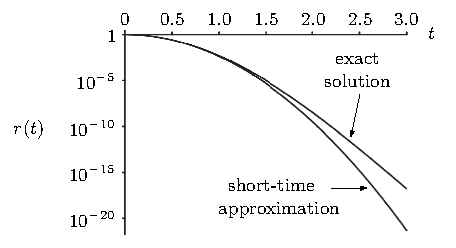
\includegraphics[width=.68\linewidth]{figures/ch05_fig05.pdf}
\caption{デコヒーレンス因子$r(t)=\langle E_-(t)|E_+(t)\rangle$、すなわち環境の相対状態の重なりの時間発展。$N=20$個の調和振動子からなる環境について、厳密な発展(5.108)と短時間近似(5.110)の両方を示した。結合$g_i$と振動数$\omega_i$は、区間$[0,1]$から無作為に選んだ。}\label{fig:5.5}
\end{figure}

% 原文 p.214
\hypertarget{srcpage:214}{}\label{srcpage:214}
系の縮約密度行列$\rho_{\mathrm S}(t)$の時間発展は、通常の方法で
\chfiveeq{114}
から得られる。$\hat V(t)$は(5.99)で与えられる。$\{|0\rangle,|1\rangle\}$基底で表した$\hat\rho_{\mathrm S}(t)$の対角要素$\rho_{\mathrm S}^{(ii)}(t)$が時間に対して一定、
\chfiveeq{115}
であることは(5.92)からすでにわかっているので、非対角要素
\chfiveeq{116}
だけを計算すればよい。上の定義を用いれば、これらは次のように容易に計算できる。
\chfiveeq{117}
言い換えれば、デコヒーレンス因子$r(t)$は
\chfiveeq{118}
で与えられる。すなわち、環境の熱モード$\hat\rho_{\mathrm E_i}$についての、演算子$\hat D(\lambda_i(t))$［(5.103)参照］の期待値の積である。

ここで
\chfiveeq{119}
は、熱平衡にある一つの調和振動子、すなわち一つの場モードの、対称順序の特性関数にすぎないことがわかる。この関数は量子光学でよく知られ（例えば文献\cite{ref241}）、次で与えられる\cite{ref018,ref150}。
\chfiveeq{120}

% 原文 p.215
\hypertarget{srcpage:215}{}\label{srcpage:215}
よって
\chfiveeq{121}
であり、指数関数の引数を$\Gamma(t)$と表した。

\subsubsectionlink*{デコヒーレンス因子の時間発展}
かなり形式的な操作を行ってきたので、次に$\Gamma(t)$を調べ、$r(t)$の時間依存性の感覚をつかもう。まず、環境が十分大きく、環境モードの連続的な密度を仮定できるとする。したがって、5.2節の量子Brown運動の議論と同様に、離散的結合$g_i$の和で表した(5.121)から、スペクトル密度$J(\omega)$による連続記述へ移る。
\chfiveeq{122}
この置換により、(5.121)の$\Gamma(t)$は
\chfiveeq{123}
となる。もちろん、
\chfiveeq{124}
を選べば、(5.123)の右辺は、自明に元の表式(5.121)と一致する。ここでは代わりに、$J(\omega)$を、適切に選んだ$\omega$の滑らかな関数で表そう。

量子Brown運動の場合（5.2.3節参照）と同様に、十分小さい振動数でOhmic、$J(\omega)\propto\omega$であり、$\Lambda$で定量化する滑らかな高振動数カットオフをもつスペクトル密度を考える。量子Brown運動模型で用いたLorentz--Drude形(5.44)の代わりに、ここでは$e^{-\omega/\Lambda}$という指数関数的なカットオフを選ぼう。したがってスペクトル密度は
\chfiveeq{125}
という形を取る。$J_0$は無次元定数である。(5.123)に現れる因子4を(5.125)へ吸収した。このスペクトル密度を図5.6に示す。意図したとおり、$J(\omega)$は$\omega<\Lambda$でほぼ線形に増加し、$\omega>\Lambda$で減少する。

$J(\omega)$の関数形(5.125)を用いると、(5.123)は
\chfiveeq{126}
となる。

% 原文 p.216
\hypertarget{srcpage:216}{}\label{srcpage:216}
\begin{figure}[htbp]\centering
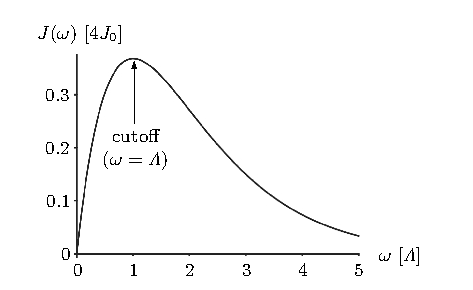
\includegraphics[width=.65\linewidth]{figures/ch05_fig06.pdf}
\caption{(5.125)で与えられるスペクトル密度$J(\omega)$（単位：$4J_0$）。スペクトル密度は、カットオフ振動数$\Lambda$より十分低い振動数では、ほぼOhmic、すなわち$J(\omega)\propto\omega$になるように選んだ。$\omega>\Lambda$では、Ohmicな性質は$e^{-\omega/\Lambda}$という項によって抑えられる。振動数$\omega$の単位はカットオフ$\Lambda$である。}\label{fig:5.6}
\end{figure}
環境の熱エネルギー$k_{\mathrm B}T$がカットオフ振動数$\Lambda$より小さい、$k_{\mathrm B}T\ll\Lambda$という妥当な仮定を置くと、この積分は厳密に解ける。結果は
\chfiveeq{127}
と分解できる。ここで
\chfiveeq{128}
は、純粋に量子的な真空揺らぎによる$\Gamma(t)$への厳密な寄与であり（浴温度に依存しないことに注意）、
\chfiveeq{129}
は、浴の熱揺らぎによる寄与である。

$\Gamma(t)$のグラフを図5.7に示す。$\Gamma(t)$は初期値1から減少する。関係するデコヒーレンス因子(5.118)は$r(t)=e^{\Gamma(t)}$なので、成分$|0\rangle$と$|1\rangle$の間のコヒーレンスは、確かに局所的に減衰すると結論できる。以下で見るように、このデコヒーレンス過程には、いくつかの特徴的な時間尺度を区別できる。

\subsubsectionlink*{デコヒーレンスの時間尺度}
二つの寄与$\Gamma_{\mathrm{fluc}}(t)$、$\Gamma_{\mathrm{therm}}(t)$のいずれかが、$\Gamma(t)$の時間発展を支配する、関係する時間尺度を調べよう。

% 原文 p.217
\hypertarget{srcpage:217}{}\label{srcpage:217}
\begin{figure}[htbp]\centering
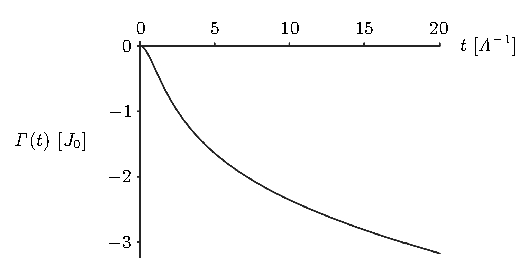
\includegraphics[width=.65\linewidth]{figures/ch05_fig07.pdf}
\caption{指数$\Gamma(t)$［(5.126)参照］の時間依存性（単位：$J_0$）。時間の単位はカットオフ周期$\Lambda^{-1}$である。浴温度は$k_{\mathrm B}T=\Lambda/60$、すなわち熱相関時間がカットオフ周期$\Lambda^{-1}$の60倍長いと仮定した。}\label{fig:5.7}
\end{figure}
(5.128)、(5.129)から、これらの時間尺度は、カットオフ周期$\Lambda^{-1}$と熱相関時間$(k_{\mathrm B}T)^{-1}$に対する$t$の大きさによって定義されるとわかる。

第一に、$t\ll\Lambda^{-1}$かつ$t\ll(k_{\mathrm B}T)^{-1}$という、極端に短い時間の領域を仮定しよう。このとき、$\Gamma_{\mathrm{fluc}}(t)$の表式(5.128)の自然対数のTaylor展開は、第2項までで打ち切れる。すなわち、$\Lambda^2t^2$の1次まで展開して、
\chfiveeq{130}
を得る。したがって$\Gamma_{\mathrm{fluc}}(t)\ll1$である。この領域では熱的寄与$\Gamma_{\mathrm{therm}}(t)$はまったく役割を果たさない。よってデコヒーレンス因子$r(t)$［(5.118)参照］は1に近く、その弱い減衰は、すべて量子的真空揺らぎによる。

第二に、$t$がカットオフ振動数で定まる特徴的周期より大きい、$t\gg\Lambda^{-1}$が、なお熱相関時間よりはるかに小さい、$t\ll(k_{\mathrm B}T)^{-1}$としよう。このときも、$\Gamma(t)$に対する$\Gamma_{\mathrm{therm}}(t)$の寄与を無視でき、$\Gamma_{\mathrm{fluc}}(t)$は
\chfiveeq{131}
と近似できる。したがって、$\Gamma_{\mathrm{fluc}}(t)$の大きさは1より大きく、この領域では量子的真空揺らぎが、支配的なデコヒーレンス源となる。

最後に、$t$が典型的な熱揺らぎ時間よりはるかに大きい長時間領域、$t\gg(k_{\mathrm B}T)^{-1}$を仮定しよう。このとき
\chfiveeq{132}
を用いると、
\chfiveeq{133}
したがって
\chfiveeq{134}
を得る。

% 原文 p.218
\hypertarget{srcpage:218}{}\label{srcpage:218}
この$\Gamma(t)$の表式を(5.121)へ代入すると、デコヒーレンス因子$r(t)$は、熱相関時間$(k_{\mathrm B}T)^{-1}$で定まる時間尺度で指数関数的に減衰することがわかる。
\chfiveeq{135}
